\chapter{Formalism}
\section{Gravitation}
	Gravity is the weakest of the four fundamental forces in our universe. Gravitation was first stated in a mathematical framework by Sir Isaac Newton in 1687 as for a particle with mass $m$ and position $\vec{r}$,
	\begin{align}
		\vec{F}=m*\vec{a}=m*G*\sum\limits_{i=0}^{N}\frac{m_i}{(r-r_i)^3}*(\vec{r}-\vec{r}_i),
	\end{align}
	where $m_i$ and $\vec{r_i}$ is the mass and position of other point masses in the universe \cite{Newton}. Modern technology has then been used to determine the gravitational constant $G = 6.67408 \cdot 10^{11} \frac{m^3}{kg \cdot s^2}$.
	
	We assume in our calculations that all planets and satellites are point-masses, which is a good approximation because they are located far away from each other and all planets are fairly spherical objects. The gravitational pull on particles outside a sphere with uniform mass distribution is equivalent to the pull of a point-mass.
	
	In our system we consider the Sun, Earth, Moon and Mars as mediators of gravitational pull, since our satellite is not heavy enough to act significantly on the other planets. For practical reasons we define $\mu\equiv G\cdot m$ for the relevant planets and stars for our systems these values are shown in \cref{tab::planetMu}
	\begin{table}[]
		\centering
		\label{tab::planetMu}
		\begin{tabular}{l|llll}
			& Sun           & Earth                           & Moon             & Mars                               \\ \toprule
			$\mu$ & $1.327124\cdot 10^{20}$ & $3986004418\cdot 10^5$ & $4.902798882\cdot 10^{12}$ & $426502472.726 \cdot 10^4$
		\end{tabular}
		
		\caption{$\mu=G\cdot m$ for relevant planets/stars}
	\end{table}

\section{Hohmann Transfer Orbit}
	To initially probe our optimization algorithm, we make an initial guess of how to fire the thrusters to end up on Mars. Hohmann Transfers are really simple to calculate, but only considers a two-body system - in this case the sun and our satellite. 
	
	\begin{figure}
		\centering
		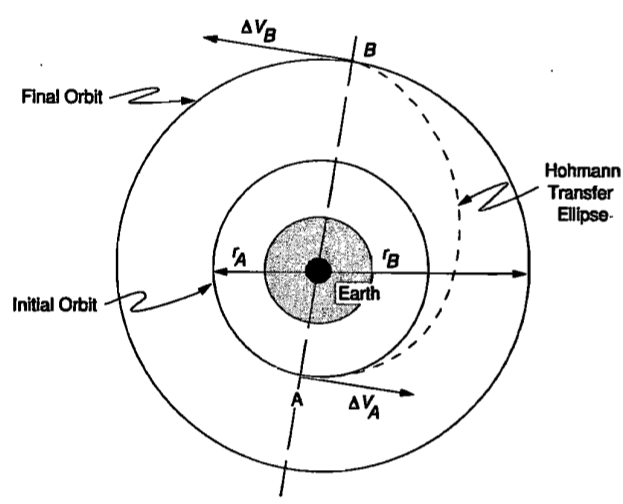
\includegraphics[width=0.5\textwidth]{hohmann}
		\label{fig:hohmann}
		\caption{Spacecraft initially located at A goes into hohmann transfer by thrusting with velocity $\Delta V_A$ and ends up in the Final Orbit at B}
	\end{figure}
\section{Numerical Solutions to Differential Equations}
\section{Optimal Control Theory}
\section{Implementing the CMA-ES Algorithm}
